\documentclass[12pt,a4paper]{article}
\title{Lab9-OpenCV}
\usepackage{ctex}
\usepackage{amsmath,amscd,amsbsy,amssymb,latexsym,url,bm,amsthm}
\usepackage{epsfig,graphicx,subfigure}
\usepackage{enumitem,balance}
\usepackage{wrapfig}
\usepackage{mathrsfs,euscript}
\usepackage[usenames]{xcolor}
\usepackage{hyperref}
\usepackage[vlined,ruled,commentsnumbered,linesnumbered]{algorithm2e}
\usepackage{float}
\usepackage{geometry}
\usepackage{listings}
\geometry{a4paper,scale=0.8}
\usepackage[T1]{fontenc}
\usepackage[utf8]{inputenc}
\usepackage{amssymb}
\usepackage{graphicx}
\usepackage{subfigure}
% --- Python code template ---
\usepackage[utf8]{inputenc}
% Default fixed font does not support bold face
\DeclareFixedFont{\ttb}{T1}{txtt}{bx}{n}{12} % for bold
\DeclareFixedFont{\ttm}{T1}{txtt}{m}{n}{12}  % for normal

% Custom colors
\usepackage{color}
\definecolor{deepblue}{rgb}{0,0,0.5}
\definecolor{deepred}{rgb}{0.6,0,0}
\definecolor{deepgreen}{rgb}{0,0.5,0}

\usepackage{listings}

% Python style for highlighting
\newcommand\pythonstyle{\lstset{
language=Python,
basicstyle=\ttm,
morekeywords={self},              % Add keywords here
keywordstyle=\ttb\color{deepblue},
emph={MyClass,__init__},          % Custom highlighting
emphstyle=\ttb\color{deepred},    % Custom highlighting style
stringstyle=\color{deepgreen},
frame=tb,                         % Any extra options here
showstringspaces=false
}}
% Python environment
\lstnewenvironment{python}[1][]
{
\pythonstyle
\lstset{#1}
}
{}

% Python for external files
\newcommand\pythonexternal[2][]{{
\pythonstyle
\lstinputlisting[#1]{#2}}}

% Python for inline
\newcommand\pythoninline[1]{{\pythonstyle\lstinline!#1!}}

% --- Python code template ---


% --- HTML lstlisting template --- %
\makeatletter
\usepackage{color}
\definecolor{lightgray}{rgb}{0.95, 0.95, 0.95}
\definecolor{darkgray}{rgb}{0.4, 0.4, 0.4}
%\definecolor{purple}{rgb}{0.65, 0.12, 0.82}
\definecolor{editorGray}{rgb}{0.95, 0.95, 0.95}
\definecolor{editorOcher}{rgb}{1, 0.5, 0} % #FF7F00 -> rgb(239, 169, 0)
\definecolor{editorGreen}{rgb}{0, 0.5, 0} % #007C00 -> rgb(0, 124, 0)
\definecolor{orange}{rgb}{1,0.45,0.13}		
\definecolor{olive}{rgb}{0.17,0.59,0.20}
\definecolor{brown}{rgb}{0.69,0.31,0.31}
\definecolor{purple}{rgb}{0.38,0.18,0.81}
\definecolor{lightblue}{rgb}{0.1,0.57,0.7}
\definecolor{lightred}{rgb}{1,0.4,0.5}
\usepackage{upquote}
\usepackage{listings}
% CSS
\lstdefinelanguage{CSS}{
  keywords={color,background-image:,margin,padding,font,weight,display,position,top,left,right,bottom,list,style,border,size,white,space,min,width, transition:, transform:, transition-property, transition-duration, transition-timing-function},	
  sensitive=true,
  morecomment=[l]{//},
  morecomment=[s]{/*}{*/},
  morestring=[b]',
  morestring=[b]",
  alsoletter={:},
  alsodigit={-}
}

% JavaScript
\lstdefinelanguage{JavaScript}{
  morekeywords={typeof, new, true, false, catch, function, return, null, catch, switch, var, if, in, while, do, else, case, break},
  morecomment=[s]{/*}{*/},
  morecomment=[l]//,
  morestring=[b]",
  morestring=[b]'
}

\lstdefinelanguage{HTML5}{
  language=html,
  sensitive=true,	
  alsoletter={<>=-},	
  morecomment=[s]{<!-}{-->},
  tag=[s],
  otherkeywords={
  % General
  >,
  % Standard tags
	<!DOCTYPE,
  </html, <html, <head, <title, </title, <style, </style, <link, </head, <meta, />,
	% body
	</body, <body,
	% Divs
	</div, <div, </div>, 
	% Paragraphs
	</p, <p, </p>,
	% scripts
	</script, <script,
  % More tags...
  <canvas, /canvas>, <svg, <rect, <animateTransform, </rect>, </svg>, <video, <source, <iframe, </iframe>, </video>, <image, </image>, <header, </header, <article, </article
  },
  ndkeywords={
  % General
  =,
  % HTML attributes
  charset=, src=, id=, width=, height=, style=, type=, rel=, href=,
  % SVG attributes
  fill=, attributeName=, begin=, dur=, from=, to=, poster=, controls=, x=, y=, repeatCount=, xlink:href=,
  % properties
  margin:, padding:, background-image:, border:, top:, left:, position:, width:, height:, margin-top:, margin-bottom:, font-size:, line-height:,
	% CSS3 properties
  transform:, -moz-transform:, -webkit-transform:,
  animation:, -webkit-animation:,
  transition:,  transition-duration:, transition-property:, transition-timing-function:,
  }
}

\lstdefinestyle{htmlcssjs} {%
  % General design
%  backgroundcolor=\color{editorGray},
  basicstyle={\footnotesize\ttfamily},   
  frame=b,
  % line-numbers
  xleftmargin={0.75cm},
  numbers=left,
  stepnumber=1,
  firstnumber=1,
  numberfirstline=true,	
  % Code design
  identifierstyle=\color{black},
  keywordstyle=\color{blue}\bfseries,
  ndkeywordstyle=\color{editorGreen}\bfseries,
  stringstyle=\color{editorOcher}\ttfamily,
  commentstyle=\color{brown}\ttfamily,
  % Code
  language=HTML5,
  alsolanguage=JavaScript,
  alsodigit={.:;},	
  tabsize=2,
  showtabs=false,
  showspaces=false,
  showstringspaces=false,
  extendedchars=true,
  breaklines=true,
  % German umlauts
  literate=%
  {Ö}{{\"O}}1
  {Ä}{{\"A}}1
  {Ü}{{\"U}}1
  {ß}{{\ss}}1
  {ü}{{\"u}}1
  {ä}{{\"a}}1
  {ö}{{\"o}}1
}
%
\lstdefinestyle{py} {%
language=python,
literate=%
*{0}{{{\color{lightred}0}}}1
{1}{{{\color{lightred}1}}}1
{2}{{{\color{lightred}2}}}1
{3}{{{\color{lightred}3}}}1
{4}{{{\color{lightred}4}}}1
{5}{{{\color{lightred}5}}}1
{6}{{{\color{lightred}6}}}1
{7}{{{\color{lightred}7}}}1
{8}{{{\color{lightred}8}}}1
{9}{{{\color{lightred}9}}}1,
basicstyle=\footnotesize\ttfamily, % Standardschrift
numbers=left,               % Ort der Zeilennummern
%numberstyle=\tiny,          % Stil der Zeilennummern
%stepnumber=2,               % Abstand zwischen den Zeilennummern
numbersep=5pt,              % Abstand der Nummern zum Text
tabsize=4,                  % Groesse von Tabs
extendedchars=true,         %
breaklines=true,            % Zeilen werden Umgebrochen
keywordstyle=\color{blue}\bfseries,
frame=b,
commentstyle=\color{brown}\itshape,
stringstyle=\color{editorOcher}\ttfamily, % Farbe der String
showspaces=false,           % Leerzeichen anzeigen ?
showtabs=false,             % Tabs anzeigen ?
xleftmargin=17pt,
framexleftmargin=17pt,
framexrightmargin=5pt,
framexbottommargin=4pt,
%backgroundcolor=\color{lightgray},
showstringspaces=false,      % Leerzeichen in Strings anzeigen ?
}%
%
\makeatother

%\begin{lstlisting}[style=htmlcssjs]
% --- HTML lstlisting template --- %


















\title{Lab11\&{12}\quad SIFT尺度不变特征变换}
\date{2021.12}
\author{孙济宸\quad \quad 学号:520030910016 \quad  \quad 班级:F2003003}
\begin{document}
\maketitle
\section{实验概览}
实现SIFT算法,测试图像匹配效果,并与OpenCV内置库比较。
使用Harris角点提取简化实现。
\section{实验环境}
\begin{itemize}
	\item OpenCV
	\item numpy
	
\end{itemize}


\section{练习题的解决思路}


\begin{enumerate}
\item 使用resize构建图像金字塔(5层)
\begin{lstlisting}[style=py]
    pyramid = []
    height, width = img.shape[0], img.shape[1]
    multipliers = [int(2 ** i) for i in range(layers)] # 0(original), /2, /4 , etc.
    pyramid.append(img)
    for i in range(1, layers):
        resized_img = cv2.resize(img,(width // 2**i, height // 2**i))
        pyramid.append(resized_img)
\end{lstlisting}
\item 对于金字塔每一层图像,首先高斯模糊,去除噪声;
\begin{lstlisting}[style=py]
img_gray = cv2.GaussianBlur(img_gray, (5, 5), 1, 1)
\end{lstlisting}
\item 提取特征点,原论文中使用DoG高斯差分金字塔寻找极值点,实验中采用OpenCV内置的goodFeaturesToTrack()方法直接获取特征点。
\begin{lstlisting}[style=py]
corners = [[int(c[0][0]),int(c[0][1])] for c in \
               cv2.goodFeaturesToTrack(image = img_gray, maxCorners = 50, qualityLevel = 0.01, minDistance = 10,  blockSize = 3, useHarrisDetector = True)]
    corners = np.array(corners)
\end{lstlisting}
\item 计算梯度大小及方向角矩阵

\item 计算描述子。对于每个特征点,通过在一个正方形邻域里统计梯度方向直方图,在36个方向上vote的方式获得主方向。
\item 在特征点的邻域内,把正方形邻域分成4*4个块,每块内再用类似主方向的统计方式在8个方向上vote,得到直方图,最后获得4*4*8=128维描述子。其中,在计算方向的时候把坐标在主方向$\theta$上进行旋转变换,以保证描述子旋转不变性。这样得到的坐标不是整数,需要进行双线性插值。
\begin{center}
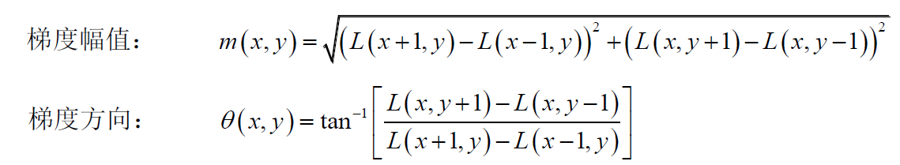
\includegraphics[width=0.8\textwidth]{grad.png}\\
\end{center}

旋转变换:
\begin{equation}
v' = \begin{pmatrix}
\cos\theta & -\sin\theta \\
\sin\theta & \cos\theta
\end{pmatrix}
v
\end{equation}
\begin{center}
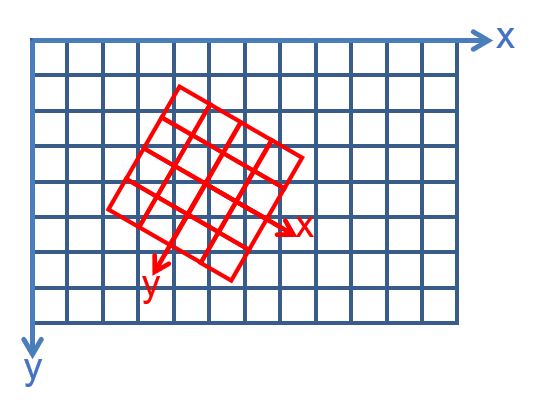
\includegraphics[width=0.5\textwidth]{rotate.png}\\
\end{center}

双线性插值:
$$
\theta(x',y') = \theta(x, y)dx_2dy_2 
                + \theta(x+1,y)dx_1dy_2 
                + \theta(x, y+1)dx_2dy_1 
                + \theta(x+1, y+1)dx_1dy_1
$$
\begin{center}
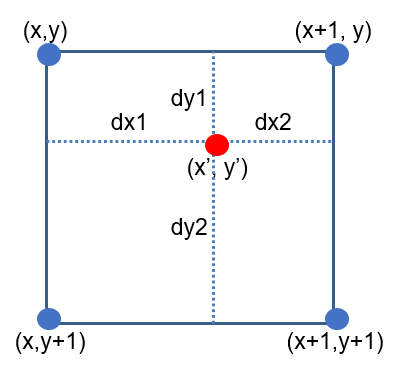
\includegraphics[width=0.5\textwidth]{dblinear.png}\\
\end{center}

代码较长见附录
\item 把图片全部特征点计算出描述子。对于金字塔的每层重复2-7, 其中角点坐标需要映射回原图的尺度。
\begin{lstlisting}[style=py]
def sift_multilayer(img): #在图像金字塔上进行sift操作
    pyramid, multipliers = calc_img_pyramid(img)
    i = 0
    all_desc = []
    all_corners = []
    for layer in pyramid:
        desc, corners = sift_singlelayer(layer)
        corners *= multipliers[i] # 把角点坐标变回原来的尺度
        i += 1
        all_desc += desc
        all_corners += list(corners)
    
    return all_desc, all_corners
\end{lstlisting}
\item 两幅图匹配时,只需对两张图的全部描述子两两匹配计算匹配度(向量点乘),大于一定阈值即可认为两点成功匹配。
\begin{lstlisting}[style=py]
def match_2imgs(merged, desc1, desc2, corners1, corners2, H, W, filename, thresh=0.8, matched_thresh=0.1):
    len1, len2 = len(corners1), len(corners2)
    matched = 0
    for i in range(len1):
        for j in range(len2):
            if np.inner(desc1[i], desc2[j]) > thresh:
                matched += 1
                 # 匹配点画圆圈和线
                color = color = ((random.randint(0, 255)), (random.randint(0, 255)), (random.randint(0, 255))) # random color
                pos1 = tuple([int(corners2[j][0]), int(corners2[j][1])])
                pos2 = tuple([int(corners1[i][0] + W), int(corners1[i][1])])
                cv2.line(merged, pos1, pos2, color=color, thickness=1)
                cv2.circle(merged, pos1, radius=5, color=color, thickness=2)
                cv2.circle(merged, pos2, radius=5, color=color, thickness=2)
    
    if matched > matched_thresh * min(len1, len2): # 匹配点数量大于10%,认为匹配到了
        cv2.imwrite(f"result_{filename}_thresh{thresh}.png", merged)
        print(f"{filename} Match! Showing result: {matched} corners matched")
        cv2.imshow(f"{filename}", merged)
        cv2.waitKey(0)
        cv2.destroyAllWindows()

    else:
        print(f"{filename} NO Match!")
\end{lstlisting}
\end{enumerate}




\section{代码运行结果}

匹配阈值=0.8

\begin{figure}[H]
\subfigure[自己实现的SIFT]{
	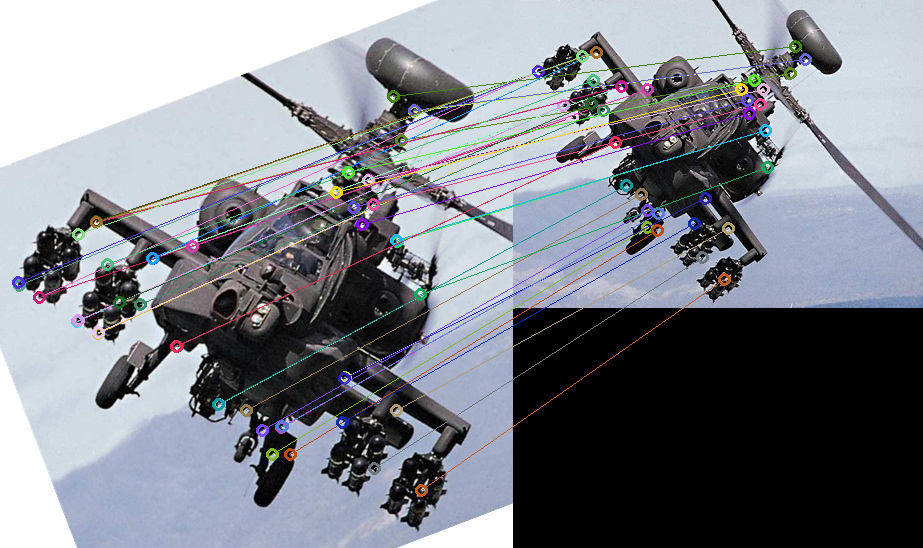
\includegraphics[width=1\textwidth]{result_3.jpg_thresh0.8.png}
	\centering
}
\subfigure[Opencv-SIFT]{
	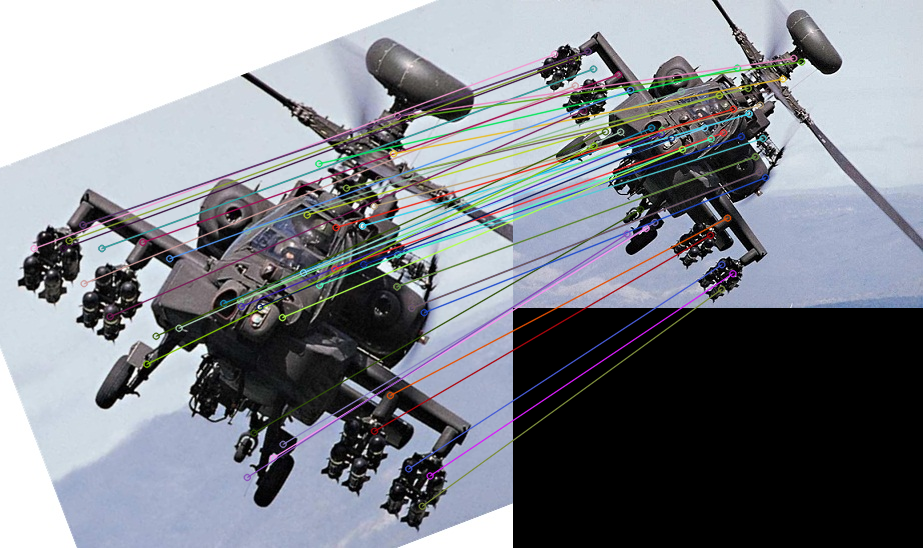
\includegraphics[width=1\textwidth]{match.png}
	
}

	


\end{figure}


\begin{figure}[H]
\subfigure[自己实现的SIFT]{
	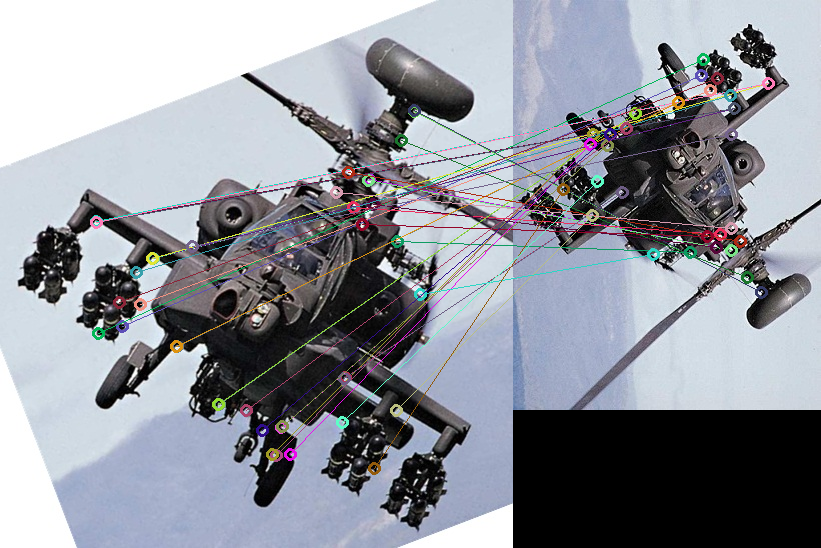
\includegraphics[width=1\textwidth]{result_6.jpg_thresh0.8.png}
	\centering
}
\subfigure[Opencv-SIFT]{
	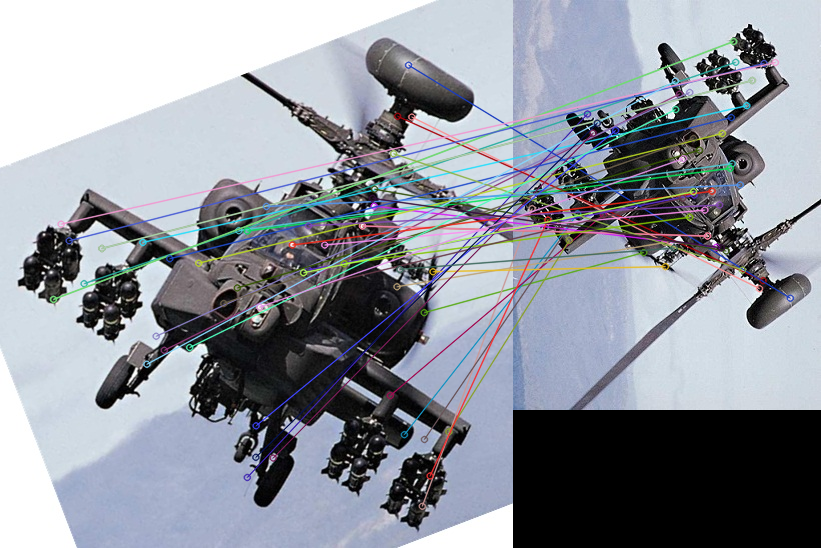
\includegraphics[width=1\textwidth]{match3.png}
	
}

	


\end{figure}

\begin{figure}[H]
\subfigure[自己实现的SIFT]{
	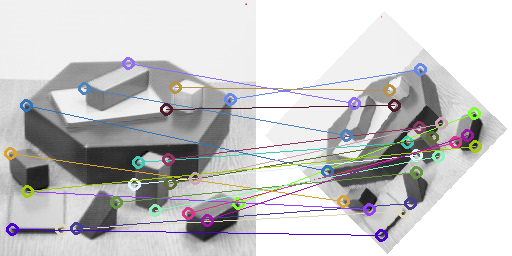
\includegraphics[width=1\textwidth]{result_7.jpg_thresh0.8.png}
	\centering
}
\subfigure[Opencv-SIFT]{
	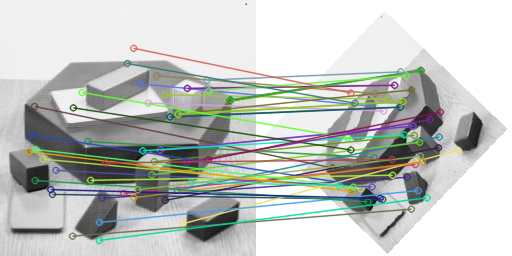
\includegraphics[width=1\textwidth]{match2.png}
	
}

	


\end{figure}

可以看出,实现的SIFT比较好地达成了尺度不变性,对图片旋转缩放都可以正确匹配,而且匹配点精确。基本达到了OpenCV库内置的效果。





\section{分析与思考}
\begin{itemize}
\item 这次实验总体比较成功,工作量很大,也在网上查阅了很多原理和代码实现方法,最终结果令人满意。
\item 由于用Harris角点提取简化了步骤,没有用高斯金字塔,在处理图像时一定要先高斯模糊,否则受噪声影响巨大。
\item 为保证SIFT描述子具有旋转不变性,在计算梯度方向和统计梯度方向直方图时需要进行一步坐标旋转变换,否则达不到效果。
\item 然而尺度不变性也导致如果一张图片上有多个相似物体,这些物体都会产生相似的描述子,导致匹配的时候其中任何一个都可能匹配上,因为算法并不会管特征点本身所处的位置,是算法本身的局限
\item 很多时候进行完数学操作必须注意numpy数组的数据类型,对于图片都是uint8,否则cv2函数可能会报错
\item 为代码实现简洁和运行效率,尽可能使用numpy和cv2库中的函数,不要自己写多重循环操作
\newpage
\end{itemize}
\section{附录:python代码}
\begin{lstlisting}[style=py]
import cv2
from cv2 import Sobel, cv2, resize # make vscode not complain
from matplotlib import pyplot as plt
import math
import numpy as np
import copy
import random

from numpy.matrixlib import mat
PI = 3.1415926

def __atan(x, y):  # return 0 ~ 2PI arctan of vector (x,y)
    return np.arctan2(y, x) if y > 0 else np.arctan2(y,x) + 2*PI

def calc_img_pyramid(img, layers=5):
    pyramid = []
    height, width = img.shape[0], img.shape[1]
    #print(height, width)
    multipliers = [int(2 ** i) for i in range(layers)] # 0(original), /2, /4 , etc.
    pyramid.append(img)
    for i in range(1, layers):
        resized_img = cv2.resize(img,(width // 2**i, height // 2**i))
        pyramid.append(resized_img)
        #cv2.imshow(str(i),resized_img)
        #cv2.waitKey(0)
        
    return pyramid, multipliers

    
def sift_singlelayer(img_gray):

    H, W = img_gray.shape[0], img_gray.shape[1]
     # Harris 获得角点
    img_gray = cv2.GaussianBlur(img_gray, (5, 5), 1, 1)
    corners = [[int(c[0][0]),int(c[0][1])] for c in \
               cv2.goodFeaturesToTrack(image = img_gray, maxCorners = 50, qualityLevel = 0.01, minDistance = 10,  blockSize = 3, useHarrisDetector = True)]
    corners = np.array(corners)
    corner_cnt = len(corners)
    # list of tuples (corner (x,y))
    #计算梯度
    gx, gy, gm, gtheta = calc_grad(img_gray)
    # 计算主方向矩阵
    main_dir = vote(corners, gm, gtheta, H, W)
    
    # 计算描述子
    #print(H, W)
    descriptors = []
    for i in range(corner_cnt):
        #print(H, W)
        desc = calc_descriptor(corners[i],  gtheta, main_dir[i], H, W)

        descriptors.append(desc / np.linalg.norm(desc)) # 归一化
    return descriptors, corners
    
def vote(corners, grad, theta, H, W):
    BINSIZE = (H + W) // 80
    main_dir = []
    for corner in corners:
        _hist = np.zeros(36)
        y, x = corner
        for i in range( max(0, x - BINSIZE), min (H, x + BINSIZE + 1)):
            for j in range( max(0, y - BINSIZE), min(W, y + BINSIZE)):
                deg10 = min( round(theta[i][j] * 18 / PI), 35 )
                _hist[deg10] += grad[i][j]
        most_deg10 = np.argmax(_hist)
        main_dir.append(( most_deg10 + 0.5 ) / 18 * PI)
    
    return main_dir


def calc_descriptor(pos, gradtheta, theta, HEIGHT, WIDTH):
    
    
    def dbl_linear(x, y): # 双线性插值
        def dtheta(x, y): # delta-theta of vector (x,y) and theta
            if (x < 0 or x >= HEIGHT) or (y < 0 or y >= WIDTH):
                return 0
            diff = gradtheta[x][y] - theta
            return diff if diff > 0 else diff + 2 * PI
        
        xx, yy = int(x), int(y)
        dy1, dy2 = y-yy, yy+1-y
        dx1, dx2 = x-xx, xx+1-x
        interpol = dtheta(xx, yy)*dx2*dy2 \
                + dtheta(xx+1,yy)*dx1*dy2 \
                + dtheta(xx, yy+1)*dx2*dy1 \
                + dtheta(xx+1, yy+1)*dx1*dy1
        return interpol

    y0, x0 = pos
    # 坐标旋转矩阵
    rotation = np.array([[math.cos(theta), - math.sin(theta)],
                        [math.sin(theta), math.cos(theta)]])

    
    def _vote(x1, x2, y1, y2, xsign, ysign):
        hist = np.zeros(8)
        for x in range(x1, x2):
            for y in range(y1, y2):
                v = np.array([x * xsign, y * ysign]).T
                _v = rotation @ v  # 旋转以后的坐标
                deg45 = int( (dbl_linear(_v.T[0] + x0, _v.T[1] + y0)) // (PI/4)) # 分成8块 8*45=360
                hist[min(deg45, 7)] += 1
        return list(hist)

    BINSIZE = (HEIGHT + WIDTH) // 128
    descriptor = []
    for xsign in [-1,1]:  # 四个象限统计
        for ysign in [-1,1]:
            descriptor += _vote(0, BINSIZE, 0, BINSIZE, xsign, ysign)
            descriptor += _vote(BINSIZE, BINSIZE * 2, 0, BINSIZE, xsign, ysign)
            descriptor += _vote(BINSIZE, BINSIZE * 2, BINSIZE, BINSIZE * 2, xsign, ysign)
            descriptor += _vote(0, BINSIZE, BINSIZE, BINSIZE * 2, xsign, ysign)
    return np.array(descriptor)


def calc_grad(img): # 计算梯度和梯度方向角度矩阵
    H, W = img.shape[0], img.shape[1]
    grad_theta = np.zeros((H, W))
    grad_M =  np.zeros((H, W))
    grad_x = cv2.filter2D(img, cv2.CV_16S, np.array([-1,0,1]).reshape(1,3))
    grad_y = cv2.filter2D(img, cv2.CV_16S, np.array([1,0,-1]).reshape(3,1))
    for i in range(H):
        for j in range(W):
            grad_theta[i][j] = __atan(grad_x[i][j],grad_y[i][j])
            grad_M[i][j] = np.sqrt(np.square(float(grad_x[i][j])) + np.square(float(grad_y[i][j])))
    return grad_x, grad_y, grad_M, grad_theta


def compare(img, merged, target_desc, target_corners, H, W, filename):
    img_desc, img_corners = sift_singlelayer(img)
    match_2imgs(merged, img_desc, target_desc, img_corners, target_corners, H, W, filename)
    
def sift_multilayer(img): #在图像金字塔上进行sift操作
    pyramid, multipliers = calc_img_pyramid(img)
    i = 0
    all_desc = []
    all_corners = []
    for layer in pyramid:
        desc, corners = sift_singlelayer(layer)
        corners *= multipliers[i] # 把角点坐标变回原来的尺度
        i += 1
        all_desc += desc
        all_corners += list(corners)
    
    return all_desc, all_corners
    
def concatenate_2imgs(img1, img2): # 把两张图横向拼接
    H1, W1 = img1.shape[0:2]
    H2, W2 = img2.shape[0:2]
    
    if H1 == H2:
        return cv2.hconcat(img1, img2)
    if H1 < H2: # 两张图不一样高的情况
        filler = np.zeros((H2-H1, W1, 3), dtype=int)
        return np.hstack([np.vstack([img1, filler]), img2]).astype(np.uint8)
    else:
        filler = np.zeros((H1-H2, W2, 3), dtype=int)
        return np.hstack([img1, np.vstack([img2, filler])]).astype(np.uint8)


def match_2imgs(merged, desc1, desc2, corners1, corners2, H, W, filename, thresh=0.8, matched_thresh=0.1):
    len1, len2 = len(corners1), len(corners2)
    matched = 0
    for i in range(len1):
        for j in range(len2):
            if np.inner(desc1[i], desc2[j]) > thresh:
                matched += 1
                 # 匹配点画圆圈和线
                color = color = ((random.randint(0, 255)), (random.randint(0, 255)), (random.randint(0, 255))) # random color
                pos1 = tuple([int(corners2[j][0]), int(corners2[j][1])])
                pos2 = tuple([int(corners1[i][0] + W), int(corners1[i][1])])
                cv2.line(merged, pos1, pos2, color=color, thickness=1)
                cv2.circle(merged, pos1, radius=5, color=color, thickness=2)
                cv2.circle(merged, pos2, radius=5, color=color, thickness=2)
    
    if matched > matched_thresh * min(len1, len2): # 匹配点数量大于10%,认为匹配到了
        cv2.imwrite(f"result_{filename}_thresh{thresh}.png", merged)
        print(f"{filename} Match! Showing result: {matched} corners matched")
        cv2.imshow(f"{filename}", merged)
        cv2.waitKey(0)
        cv2.destroyAllWindows()

    else:
        print(f"{filename} NO Match!")


if __name__ == "__main__":

    target = cv2.imread(r"target.jpg")
    imgs = [cv2.imread(f"./dataset/{i}.jpg") for i in range(1,6)]
   
    target_gray = cv2.cvtColor(target, cv2.COLOR_BGR2GRAY)
    imgs_gray = [cv2.cvtColor(img, cv2.COLOR_BGR2GRAY) for img in imgs]  # 转化为灰度图

 
    target_desc, target_corners = sift_multilayer(target_gray)
    H, W = target.shape[0:2]
    for i, img_gray in enumerate(imgs_gray):
        merged = concatenate_2imgs(target, imgs[i])
      
        compare(img_gray, merged, target_desc, target_corners, H, W, str(i+1)+'.jpg')





\end{lstlisting}
\section{Reference}
\noindent
https://zhuanlan.zhihu.com/p/157578594\\
https://www.pythonheidong.com/blog/article/301412/de52ba77b3331350ccb7/\\
https://zhuanlan.zhihu.com/p/102272392\\
https://www.pythonf.cn/read/86508\\
https://blog.csdn.net/abcjennifer/article/details/7639681\\
\end{document}



